\documentclass{scrartcl}
\usepackage{german}
\usepackage[utf8]{inputenc}
\usepackage[german]{babel}

% zusätzliche mathematische Symbole, AMS=American Mathematical Society
\usepackage{amssymb}
\usepackage{amsmath}
% fürs Einbinden von Graphiken
\usepackage{graphicx}

% für Namen etc. in Kopf- oder Fußzeile
\usepackage{fancyhdr}

% erlaubt benutzerdefinierte Kopfzeilen
\pagestyle{fancy}

% Definition der Kopfzeile
\lhead{
\begin{tabular}{lllll}
Nils Hagner & 4346038 & Felix Karg & 4342014 \\
Michael Fleig & 4340085 & Anush Davtyan &4368689
\end{tabular}
}
\chead{}
\rhead{\today{}}
\lfoot{}
\cfoot{Seite \thepage}
\rfoot{}

\begin{document}

\section*{Solutions for Excercise sheet 2}

\subsection*{Exercise 1 – OCL}

\begin{itemize}
        \item[i]
        $\mathcal{S} = (\{Int\}, {TreeNode, Object}, \{key : Int, left\_Child : TreeNode, right_Child : TreeNode, parent : TreeNode, value : Object \}, \{TreeNode\mapsto \{key, left\_Child, right\_Child, parent, value\}, Object\mapsto \{\}\},
        \{\}, \{TreeNode\mapsto \emptyset, Object\mapsto \{\}\})
        \mathcal{D}(Int) = Z,
        \mathcal{D}(TreeNode) = \{T1, T2, T3, ...\},
        \mathcal{D}(Object) = \{O1, O2, O3, ...\}$
        \item[a)]
        \begin{align*}
                \sigma_{1} = \{
                &T_{1}\mapsto \{key\mapsto 20,
                left\_Child \mapsto \{T2\},
                right\_Child \mapsto \{T3\},
                parent \mapsto \emptyset,
                value \mapsto O_1
                \}\\
                &T_{2}\mapsto \{key\mapsto 10,
                left\_Child \mapsto \emptyset,
                right\_Child \mapsto \emptyset,
                parent \mapsto \{T1\},
                value \mapsto O_2
                \}\\
                &T_{3}\mapsto \{key\mapsto 20,
                left\_Child \mapsto \emptyset,
                right\_Child \mapsto \emptyset,
                parent \mapsto \{T1\},
                value \mapsto O_3
                \}\\
                &O_1\mapsto \{\}\\
                &O_2\mapsto \{\}\\
                &O_3\mapsto \{\}\\
                \}
        \end{align*}
        \includegraphics*[scale=0.5]{1a.png}\\
        The system state $\sigma_{1}$ evaluates to true because $key(left\_Child(T_{1})) \leq key(T_{1}) \leq
        key(right\_Child(T_{1}))$
        \newpage
        \begin{align*}
        \sigma_{2} = \{
        &T_{1}\mapsto \{key\mapsto 20,
        left\_Child \mapsto \{T2\},
        right\_Child \mapsto \{T3\},
        parent \mapsto \emptyset,
        value \mapsto O_1
        \}\\
        &T_{2}\mapsto \{key\mapsto 10,
        left\_Child \mapsto \emptyset,
        right\_Child \mapsto \emptyset,
        parent \mapsto \{T1\},
        value \mapsto O_2
        \}\\
        &T_{3}\mapsto \{key\mapsto 10,
        left\_Child \mapsto \emptyset,
        right\_Child \mapsto \emptyset,
        parent \mapsto \{T1\},
        value \mapsto O_3
        \}\\
        &O_1\mapsto \{\}\\
        &O_2\mapsto \{\}\\
        &O_3\mapsto \{\}\\
        \}
        \end{align*}
        \includegraphics*[scale=0.5]{1b.png}\\
        The system state $\sigma_{2}$ evaluates to false because \\ $key(left\_Child(T_{1})) < key(right\_Child(T_{1})) = key(T_{1})$

        \begin{align*}
        \sigma_{3} = \{\}
        \end{align*}
        The system state $\sigma_{3}$ evaluates to $\perp$ because there are no Instances of TreeNode and the formula can not be evaluated to true or false.

    \item[iii]
    \item[a)] $ \forall o \in allInstances_{Object} \bullet \forall t_1 \in allInstances_{TreeNode} \bullet \forall t_2 \in allInstances_{TreeNode} \bullet (value(t_1) = o \Rightarrow value(t_2) \neq o)$ \\
    \item[b)] $ \forall t_1 \in allInstances_{TreeNode} \bullet \forall t_2 \in allInstances{TreeNode} \bullet (t_1 = leftChild(t_2) \Leftrightarrow t_2 = parent(t_1))$ \\ \\
        Some System States: \\
        \newpage
        (Working for Both) $\sigma_1:$ \\
        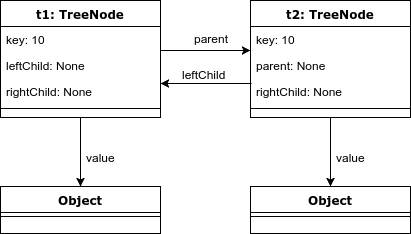
\includegraphics[width=\textwidth]{Working.png} \\
        (Failing for Both) $\sigma_2:$ \\
        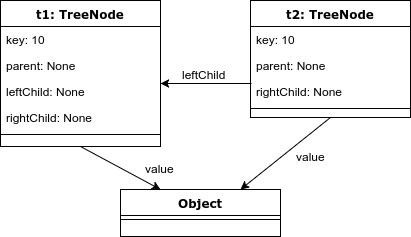
\includegraphics[width=\textwidth]{Failing.png} \\

\end{itemize}

\subsection*{Exercise 2}
Uppaal-checks: \\
E<> worker.BROKEN \\
(Property is Satisfied)
E<> (P1.CRITICAL \&\& P2.CRITICAL) \\
(Property is Satisfied)


\subsection*{Exercise 3}

A[] not ((Process(0).CRITICAL + Process(1).CRITICAL + Process(2).CRITICAL + Process(3).CRITICAL) > 1) \\
(or generally from 0 to n)

A and B do not satisfy the Mutual exclusion.

\end{document}
